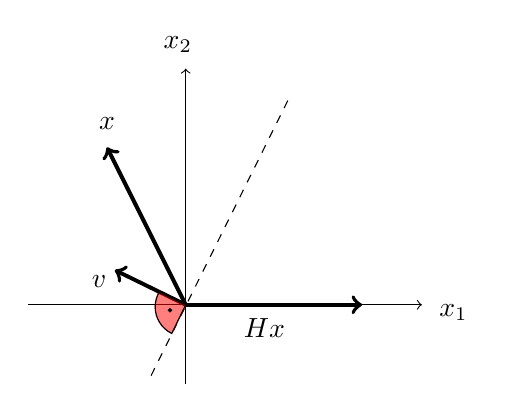
\begin{tikzpicture}

\draw[->] (-2,0) -- (3,0);
\draw[->] (0,-1) -- (0,3);

\draw[->,line width=0.5mm] (0,0) -- (-1,2);
\draw[->,line width=0.5mm] (0,0) -- (2.24,0);

\draw[dashed] (-0.44,-0.9) -- (1.34,2.68);
\draw[->,line width=0.5mm] (0,0) -- (-0.9, 0.44);




%Rechter Winkel
\filldraw[red, opacity=0.5] (0,0)--(-0.3375, 0.16) arc (150:244:.375cm) -- (0,0) ;
\draw[black, opacity=1] (0,0)--(-0.3375, 0.16) arc (150:244:.375cm) -- (0,0) ;
\filldraw(-0.2,-0.07) circle (.02cm) ;

%Beschriftung
\draw (3.4,-0.1) node {$x_1$};
\draw (-0.1,3.3) node {$x_2$};

\draw (-1.1, 0.3) node {$v$};
\draw (-1, 2.3) node {$x$};
\draw (1,-0.3) node {$Hx$};


\end{tikzpicture}